\documentclass[letterpaper]{article}

\usepackage{natbib,alifeconf}
\usepackage{amsmath}
\usepackage{mathtools}  
\mathtoolsset{showonlyrefs} 

\title{Innovation dynamics in multi-scalar systems of cities}

\author{Juste Raimbault$^{1,2,3,4}$ \and Denise Pumain$^{4}$\\
\mbox{$^1$ LASTIG, Univ. Gustave Eiffel, IGN-ENSG}\\
\mbox{$^2$ CASA, UCL}\\
\mbox{$^3$} UPS CNRS 3611 ISC-PIF\\
\mbox{$^4$ UMR CNRS 8504 G{\'e}ographie-cit{\'e}}s\\
juste.raimbault@ign.fr}

% $^*$Each submission will undergo a double-blind review process. To this end, submissions should NOT contain any element that could reveal \\ the identity of the authors (author names, affiliations, funding details and acknowledgments), and should use the third person to refer to \\ previous work by the authors. These notes should be removed/commented out, but please remember that the page limit will remain, strictly, \\8 pages (not including citations) in case of acceptance, with mandatory name(s), affiliation(s), and email address of a corresponding author. \\


\begin{document}
\maketitle

\begin{abstract}
% Abstract length should not exceed 250 words
Innovation dynamics in social and technological systems are strongly linked to urban systems and their multi-scale properties. Understanding underlying processes is crucial for sustainable territorial planning. We introduce a multi-scalar model for innovation dynamics in systems of cities, coupling a macroscopic innovation diffusion and urban dynamics model with mesoscopic models for local innovation clusters. The model parameter space is explored, and we apply a bi-objective optimisation algorithm with objectives across scales. Implementing indicators for downward causation, we finally investigate with a diversity search algorithm the diverse regimes of emergence the model can produce. This suggests strong emergence is captured, confirming the relevance of multi-scale approaches to artificial societies and urban simulation.
\end{abstract}

% keywords
% innovation dynamics
% urban simulation
% multi-scale modelling
% model validation


\section{Introduction}


Innovation is defined for social systems as inventions that became socially accepted, generating increasing returns and path dependence effects in territorial development \citep{arthur1994increasing}. Although inventions are not necessarily generated within cities, the processes of appearance and transmission of innovations are closely linked to urban development. Innovation and urban systems are thus two distinct dimensions of the Sustainable Development Goals which are tightly interlinked \citep{hegre2020synergies}. In a recent plea for better coordination of international development policies, \cite{keith2022new} emphasise that cities are drivers for the development of climate resilient approaches. Cities are complex adaptive systems whose size and functional specialization depend on their cumulative adaptation to the innovation they contribute to generate \citep{pumain2020theories}. Innovation remains rather highly geographically concentrated in an early stage before it becomes widely imitated and disseminated \citep{audretsch1996innovative}. Innovation clusters are indeed important components of local urban systems \citep{moreno2006innovation}. Spatial proximity favour local synergies, it supports knowledge spillover that may increase the spatial concentration and sustainability of innovation, provided that a related variety among local activities can help it \citep{boschma2009related,frenken2007related}.

The scale of innovation processes became much more international in recent decades. Nowadays, the acceleration of global innovation is driven by two complementary processes: the action of major players such as multinational companies in their networks \citep{rozenblat2007firm}, and the connection of resources (such as knowledge, market access, financial investment and technology legitimacy) that had previously only been brought into contact to a limited extent. Systems of cities play a crucial role in innovation processes because of the multiple interactions they have developed over time \citep{scott2015nature}. Cities sizes inequalities are prone to enable complementarities that are helping the hierarchical diffusion of innovation \citep{hagerstrand1968innovation}. As confirmed by recent investigations in urban scaling laws \citep{pumain2006evolutionary}, innovative activities at first concentrate in higher levels of urban hierarchies where skills and diversity are maximised, in a second stage they relocate in medium size cities where labour and housing market are less expensive and in a third stage relatively concentrate in smaller places. Thus in general innovation diffusion dynamics imply multiple scales. Besides the multiple observations of local innovative milieu, and the quest for global innovation systems \citep{binz2017global}, there is a regionalisation process that encourage developmental transnational partnerships between countries that belong to different regions of the world experimenting similar problems, as in the EU \citep{palle2022multilevel} or ASEAN in South Asia \citep{krapohl2017regional}. \cite{binz2017global} suggest a typology of global innovation systems based on the type of linkages within and between scales, from the regional to the global one, with different policy implications to encourage green technologies. \cite{bauer2019local} show that the interplay between local innovation and global trends is crucial for the clean transition of chemical industries.

Multi-scalar approaches are therefore necessary for innovation policies and governance. Modelling and simulation are in that context a privileged tool to understand system dynamics and elaborate policies. \cite{rozenblat2018conclusion} emphasise the need for multi-scalar models for sustainable territorial policies. The field of artificial life (ALife) has an important contribution record to the simulation of social systems, including for example the stock market \citep{palmer1994artificial}, social interactions \citep{sawyer2003artificial}, sustainable cities \citep{wang2004artificial}. One advantage of such ``artificial societies'' approaches is that they provide some explanatory power through their generative aspect \citep{grune2009explanatory}. The quantitative study of cities and urban systems has always kept tight links with ALife \citep{raimbault2020cities}. Recent urban simulation examples include the simulation of urban morphology \citep{raimbault2019generating} or informal innovation diffusion in firm clusters \citep{raimbault2022innovation}. Multi-scale models have also been proposed in that context, such as by \cite{raimbault2021strong} which couple population dynamics in a system of cities with local urban form dynamics. \cite{raimbault2021multiscale} simulates building evolution at one scale and transportation network dynamics at one other. \cite{rojas2021sustainability} introduces a network model for the diffusion of renewable energy technologies with applications at multiple scales. \cite{torrens2012polyspatial} use agents which can act at different scales to capture multi-scalar aspects of urban growth. Urban climate is also an aspect requiring highly resolved local models which can be integrated into broader meteorological models \citep{mauree2018multi}. Other aspects of social interactions, such as epidemiological modelling, are also cases where coupling between scales allows refining macroscopic equation models \citep{banos2015importance}. In the case of urban dynamics modelling, the diversity of processes and actors acting at distinct scales makes it complicated to build multi-scalar models (need for distinct ontologies and specific processes to capture the feedback between scales \citep{raimbault2021strong}), on the contrary to other types of system where the links are more explicit such as traffic \citep{banos2017multiscale}.

This paper proposes to investigate a social simulation approach to multi-scalar innovation dynamics in systems of cities. We study how the macroscopic scale of regional systems can be articulated with the mesoscopic scale of urban areas, for the emergence of new innovations within research clusters and the diffusion of these innovations between cities. We focus on the feedback between scales, the autonomy of each scale, and the need to build such a ``complicated'' model to capture strong emergence. Our contribution relies more precisely on the following: (i) we build a multi-scalar agent-based model for innovation dynamics, by coupling an innovation cluster model with an urban dynamics model at the macroscopic scale - based on existing models which have been modified and extended with some coupling processes between scales - and that we apply on synthetic systems of cities with a realistic geographical setting; (ii) we explore the coupled model parameter space using the OpenMOLE platform for model validation, including a bi-objective optimisation between utility at the macro scale and diversity at the meso scale; (iii) we implement indicators to quantify downward causation in order to understand the complexity of inter-scale interactions; (iv) we apply a diversity search algorithm to find how flexible the model is to generate ``regimes of emergence''.

The rest of the paper is organised as follows: we first formally describe the simulation model and its parametrisation; we partly validate the model by sampling its parameter space to study its statistical properties and indicator behaviour; we then run a bi-objective optimisation to find compromise between objectives at different scales; we describe the regimes of emergence obtained with the diversity search algorithm; we finally discuss the implications of our results and perspectives open for future work.


\section{Multi-scalar innovation dynamics model}

\subsection{Model rationale}

Our main hypothesis to build this model is that two distinct scales and dynamics, strongly coupled through bottom-up and top-down feedback, are necessary to capture the whole complexity of innovation systems. At the macroscopic scale of systems of cities, important related processes are the hierarchical diffusion of innovations between urban areas \citep{hagerstrand1968innovation} and the economic specialisation of these areas. \cite{favaro2011gibrat} proposed an urban dynamics model focusing on innovation diffusion, which was extended into an urban evolution model by \cite{raimbault2020model}. At the mesoscopic scale of innovation clusters, firms interact directly but also informally, and the innovation dynamics within a local area will be driven, beside numerous economic factors, by the exchange of ideas and research dynamics within and between firms (including academic bodies). \cite{raimbault2022innovation} introduced a simple model of firm clusters, accounting for geographical structure and the flow of ideas between firms, similar to a biogeography optimisation algorithm \citep{simon2008biogeography}. The multi-scale model we propose is based on a strong coupling between the macroscopic agent-based model of \cite{raimbault2020model} and the mesoscopic agent-based model of \cite{raimbault2022innovation}. Innovations diffuse within an urban system with several urban areas, in which firms search for new innovations. To simplify, urban areas are isolated enough so that no innovation cluster extends on two distinct areas (what is geographically reasonable for most worldwide urban systems, besides polycentric mega-city regions- which should in our case be considered as a single urban area \citep{yeh2020cities}). We assume a certain independence between the macro and meso dynamics, as they have each their own processes: innovation diffusion, adoption by the population, urban migration and growth, for the macro-scale; and flows of ideas within and between firms, mutation of ideas, multi-dimensional problem solving, for the meso scale. The link between scales is ensured through a bottom-up feedback: fitness performances of a local cluster, within a local innovation cycle corresponding to a macro time step, will determine the emergence of new innovations (replacing the mutation mechanism of the urban evolution model of \cite{raimbault2020model} we integrate); and through a top-down feedback: after a macro time-step, city population growth - interpreted as a global performance proxy - will have an impact on the strategies of firms and on the local urban environment, what is captured by a modification of parameter values of mesoscopic models.


\subsection{Model description}

\subsubsection{Model agents and setup}

At the macroscopic scale, agents in the model are $N$ urban areas indexed by $i$, characterised by their population $P_i(t)$ evolving with time $t\geq t_0$ and innovation genome $\delta_{ic}(t)$ which corresponds to the share of different innovations (indexed by $c$) adopted in each area. For the geographical configuration, we work on synthetic systems of cities with realistic properties, what allows exploring model behaviour independently of geographical contingencies \citep{raimbault2019space}. Initial cities sizes in terms of population follow a rank-size law (Zipf's law) $P_i = P_0 \cdot i^{-\alpha^P}$, with $P_0$ the size of the largest city, $i$ the rank in decreasing order, and $\alpha_P$ the hierarchy \citep{ioannides2003zipf}.

The mesoscopic geographical scale corresponds to the internal representation of each area, which consists in a cluster of firms. The number of firms $N_i$ in each area scales with city size \citep{pumain2006evolutionary}, such that $N_i = N_0 \cdot \left(\frac{P_i (t_0)}{P_0 (t_0)}\right)^{\alpha_N}$. We furthermore consider a global rank-size law for the size of firms (number of employees), in accordance with the empirical literature \citep{axtell2001zipf}, given by $S_k = S_0 \cdot k^{- \alpha_S}$, where $k$ is sorted in decreasing order, and such that $1 \leq k \leq \sum_i N_i$. To distribute initial firms into the urban areas: (i) we assume that the size of the largest firm scales with city size $\max_{k\in i} S_k = S_0 \cdot k^{- \alpha_L}$; (ii) sampling the set of all firms previously generated, we select for each area its largest by choosing the one with a size closest to the one given by the previous law; (iii) remaining missing firms are uniformly drawn within the sample of firms smallest than the largest, starting with the smallest urban area such that all firms are distributed in the end.

Each innovation cluster is initialised with random employees within each firm (an employee corresponding to a set of ideas, i.e. a multidimensional genome), and with a random fitness to maximise following \cite{raimbault2022innovation} given by a generalised Rastrigin function $y(\vec{x}) = - \sum_{i,j} m_{ij} \left[x_i^2 - 10 \cos\left(2 \pi x_i\right) \right] $ for an employee ideas $\vec{x}$ and $m_{ij}$ uniformly drawn random coefficients. Such difficult optimisation landscapes have been used in the literature as a proxy of what firms seek to optimise. Firms have uniformly distributed locations within each area. Each area has its own meso parameters (listed below), initialised at the same value but evolving in different ways with the macro trajectory of the city.


\subsubsection{Model dynamics}

The dynamics are simulated in an iterative way, starting from the initial state described above. For a certain number $t_f$ of macroscopic time steps, the following sequence is followed:

\begin{enumerate}
\item \textbf{Meso cycle:} each urban area (corresponding to one innovation cluster) undergoes one cycle of innovation: for $t_m$ mesoscopic time steps, after all employee ideas and the problem to solve have been randomly reinitialised:
    \begin{itemize}
        \item employee exchange ideas within firms, through crossovers between genomes with a probability $p_C$ and a share of genome exchanged $s_C$; ideas are mutated with a probability $p_M$ and amplitude $x_M$;
        \item fitness of new ideas is evaluated on the problem to maximise, and the best idea is chosen as new candidate product by the company (and attributed to a share $s_P$ of employee to work on);
        \item ideas are informally exchanged between firms within the urban area through daily life and the urban environment, following a spatial interaction model with probability $p_E$ and spatial range $d_E$.
    \end{itemize}
\item \textbf{Bottom-up feedback:} the innovations obtained in firms are put to the market if they reach a high enough quality. Considering for each area the relative fitness gain $\delta f_i = \frac{\max_k f_k - \bar{f}}{\bar{f}}$ with $\bar{f}$ the average of $f_k$ (fitness of firms), a new innovation emerges at the macroscopic scale in the corresponding urban area if this relative gain exceeds a parameter threshold $\delta f_i > \theta_i$; the list of innovative cities is transmitted to the macro scale.
\item \textbf{Macro step:} a standard step of the macroscopic model is achieved following \cite{raimbault2020model}, except for the mutation as new innovations are already simulated through the meso scale:
        \begin{itemize}
            \item innovation are diffused between cities, following
            \[\delta_{ic}(t) = \frac{\sum_j p_{cj}(t-1)^{\frac{1}{u_c}} \cdot \exp{(-\frac{d_{ij}}{d_I})}}{\sum_c \sum_j p_{cj}(t-1)^{\frac{1}{u_c}} \cdot \exp{(-\frac{d_{ij}}{d_I})}}\] with $d_I$ innovation diffusion spatial span, $u_c$ utility of the innovation $c$, $p_{jc}$ the share of adoption of $c$ in city $j$;
            \item migration and population growth are captured by the intermediary of city attractivity (determined by its innovation), such that
            \begin{equation}
            \begin{split}
            P_i(t) - P_i(t-1) \propto & w_I \cdot \sum_j \frac{P_{i}(t-1) \cdot P_{j}(t-1)}{(\sum_k P_k(t-1))^2}\\
            & \cdot \exp{\left(-\frac{d_{ij}}{d_G}\right) \cdot \prod_c \delta_{c,i,t}^{\phi_{c}(t)}}
            \end{split}
            \end{equation}
            with $\phi_c$ macro adoption levels, $d_G$ migration range parameter, $w_I$ weight parameter, and with a renormalisation by the average of gravity potentials (note the typo in \citep{raimbault2020model}: attractivity factors are indeed outside the exponential);
            \item innovative cities obtained from the meso-scale introduce new innovations, with an initial penetration rate $r_0$, and with a log-normal distributed random utility with average the current average of utilities and standard deviation a parameter $\sigma_U$ (the link between meso performance and macro utility is not endogenous, as it would require much more elaborated modelling of market processes).
        \end{itemize}
\item \textbf{Top-down feedback:} we consider two different processes through which macro dynamics will influence the next meso innovation cycles, in a way similar to \cite{raimbault2021strong}; given the relative population growth of cities at the macro scale $\delta p = \frac{P_i(t)-P_i(t-1)}{\max_j P_i(t)-P_i(t-1)}$, we assume that this captures a dynamic urban environment with consequences on firm strategy and local exchanges (we do not consider in this top-down feedback the other main process of the macro model, which are innovation share dynamics; once again the underlying economic processes are too broad to link these with city global integration and performance);
    \begin{itemize}
        \item firm strategy is updated by changing crossover probability (organisation of R\&D teams) and mutation probability (access to resources) following \[p_C(t+1,i) = p_C (t,i)\cdot (1+ \beta_C \delta_p)\] and \[p_M(t+1,i) = p_M (t,i)\cdot (1+ \beta_M \delta_p)\] - a positive value for the $\beta_C$ parameter (resp. $\beta_M$) will mean that the company follows the city trend (more intensive research in growing area and less in stagnating ones), while a negative value will imply an inverse strategy (large research centres in less dynamic areas - which can occur for many other economic, geographical and social reasons, including policy incentive to redevelop such areas);
        \item the urban environment, in terms of informal exchanges, is also influenced in a similar way following
        \[p_E(t+1,i) = p_E (t,i)\cdot (1+ \beta_E \delta_p)\]
    \end{itemize}
\end{enumerate}

The model is stopped when the final number of time steps is reached, and indicators are computed at the meso and macro levels on full trajectories.


\subsubsection{Model indicators}

% indicators / experiments
% - firm utility vs social utility
% - emissions ? (sdg approach? ~ - too far) : for contradictory optim? or between levels with utilities?
% - downward causation test
% meso diversity / best fitness: last of cycle only

We consider as observables at the macro scale the same indicators as used by \cite{raimbault2020model}: average utility $U$ (in time and across cities and innovations, weighted by population), average diversity $D$ of adoption proportions, and number of innovations. At the meso scale, we aggregate firm trajectories within each area with some indicators from \citep{raimbault2022innovation}: $f_i$ the value of the best fitness across all firms for area $i$, and $d_i$ the diversity of ideas within each area. Both are also averaged across areas to yield scalar observables $f$ and $d$.

Crucial indicators to answer our research question must be some proxy to measure ``the strength of emergence'', in some sense a quantification of downward causation. \cite{seth2010measuring} has introduced a measure based on Granger causality to estimate how the macro observables of a system are autonomous of underlying micro causal structures. \cite{rosas2020reconciling} generalise this approach by using information theory to introduce a quantitative definition of downward causation. We use the three indicators for large systems introduced by \cite{rosas2020reconciling}. Given a time-series of a macro observable $V(t)$ and of meso observables $X_j(t)$, $I(X;Y)$ an estimator of mutual information, and $\tau$ a time delay, the system exhibits causal emergence if $\Psi = I(V(t); V(t+\tau)) - \sum_j I(X_j(t) ; V(t+\tau)) > 0$. The presence of downward causation is obtained when $\Delta = \max_j \left(I(V(t) ; X_j(t+\tau)) - \sum_i I(X_i (t) ; X_j(t+\tau)) \right)$. Finally, causal decoupling is observed when $\Psi > 0$ and $\Gamma = max_j I(V(t) ; X_j (t + \tau)) = 0$. We estimate these indicators on time-series for meso observables at the level of cities $(f_i,d_i)(t)$ with the time-series for utility and diversity macro observables.


\section{Results}


\subsection{Model implementation}

The simulation model is implemented in \texttt{scala} for performance purposes. The JIDT java library is used to estimate mutual information for the downward causation indicators \citep{lizier2014jidt}. The model is integrated into the OpenMOLE platform for model exploration and validation \citep{reuillon2013openmole}, which provides a transparent access to high performance computing environments and state-of-the-art sensitivity analysis and validation methods. Model source code and analysis of simulation results are available on an open git repository at \texttt{https://github.com/JusteRaimbault/}\\\texttt{InnovationMultiscale-model}.


\subsubsection{Model parametrisation}

%\subsubsection{Model parameters}
% Macro : innov diff : d_I, d_G, beta, alpha_I, sigma_U, r_0
% Meso : ~ biogeo optim : alpha_S firms ; (p_C,s_C crossover) ; (p_M, x_M) mutation ; s_P ; (p_E, d_E) exchanges
% boundary for largest firm size: r&d unit
% fixed parameters / varying


We fix a certain number of parameters linked to geography and the configuration of the economic system, as our main research question is to focus on inter-scale relationships. Regularities of city systems are in our case fixed through the synthetic setup parameters, but each model repetition imply a different random configuration and hence some conclusions relatively independent of geographical contingencies \cite{raimbault2019space}. We consider $N=10$ cities, with maximal population $P_0 = 10000$ and hierarchy $\alpha_P = 1.0$ - these are classical settings for such regional systems of cities. This corresponds to a time scale of $t_f = 50$, roughly 50 years in reality. Meso time steps are set to $t_M=50$, corresponding to the scale of a week, typical of development sprints. Firm size scaling is also standard with $\alpha_S = 1.0$ and the size of the largest firm $S_0 = 100$ (to be interpreted in terms of R\&D team size). The number of firms for the largest area is $N_0 = 20$ and the scaling of firm number is $\alpha_N = 1.0$.

Beside these geo-economic setup parameters, we fix other parameters which are known to have limited qualitative influence on behavior of submodels from previous explorations, or which do not correspond to a process in focus. We take for the macro level $w_I = 0.01$ for a steady but limited growth, an early adopters rate $r_0=0.2$, a utility standard deviation of $\sigma_U = 1.0$. For meso clusters, fixed parameters are the genome size $g=10$, the crossover share $s_C=0.5$, the mutation amplitude $x_M=1.0$, the product share $s_P=0.5$, and the exchange spatial range $d_E = 100.0$.

The parameter left free and that will be explored in the numerical experiments are: the macro spatial interaction range $d_G$ and innovation diffusion range $d_I$, to study spatial properties of the system; the meso crossover probability $p_C$, mutation probability $p_M$ and interaction probability $p_E$, to study the role of local knowledge exchanges; and the inter-scale parameters which are at the core of our research question: $\theta_i = \theta$ innovation threshold, taken as uniform over all urban areas, and macro-to-meso feedback parameters $\beta_C$, $\beta_M$ and $\beta_E$. Parameter ranges are taken from previous exploration of the models integrated; between 1.0 and 2.0 for $\theta$ (obtained with empirical tests), and 10 times smaller than corresponding parameter boundaries for the feedback parameters to ensure a reasonable variation across the full model execution.


\begin{figure*}
    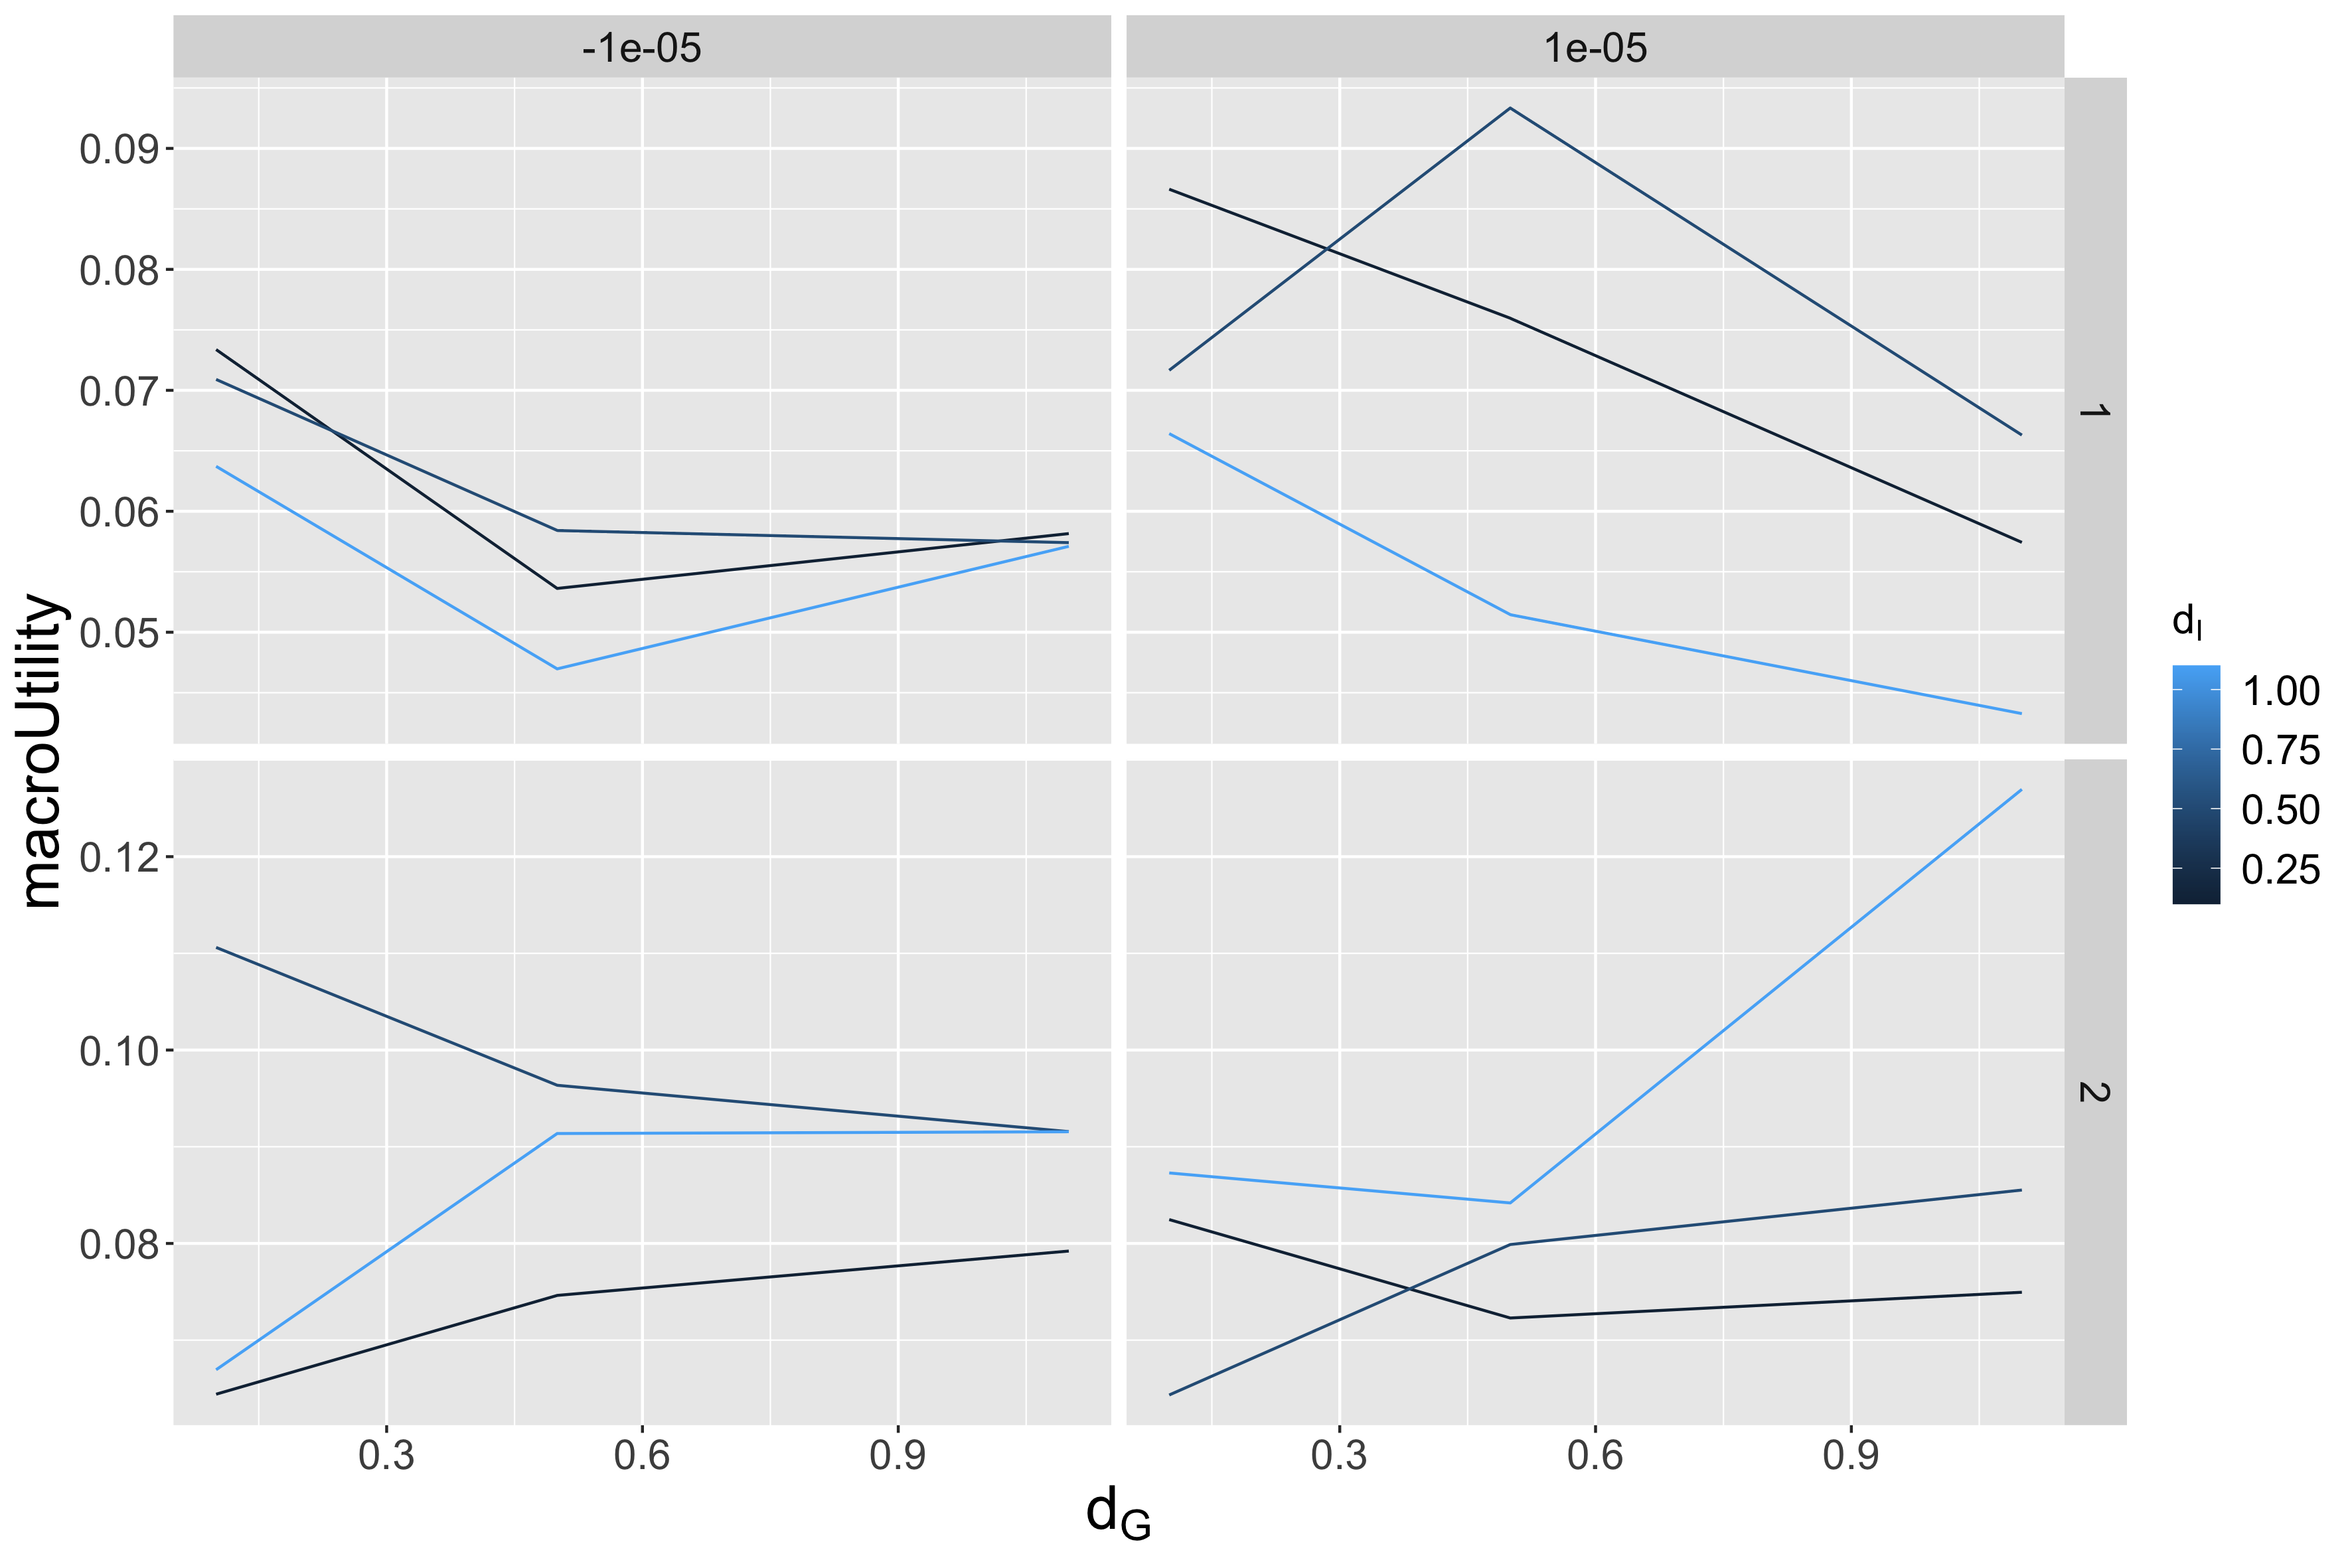
\includegraphics[width=\linewidth]{figures/macroUtility-macroGravityDecay_color-macroInnovationDecay_facet-mesoToMacroInnovationThreshold-macroToMesoExchangeMaxUpdate_mesoCrossOverProba05.png}
    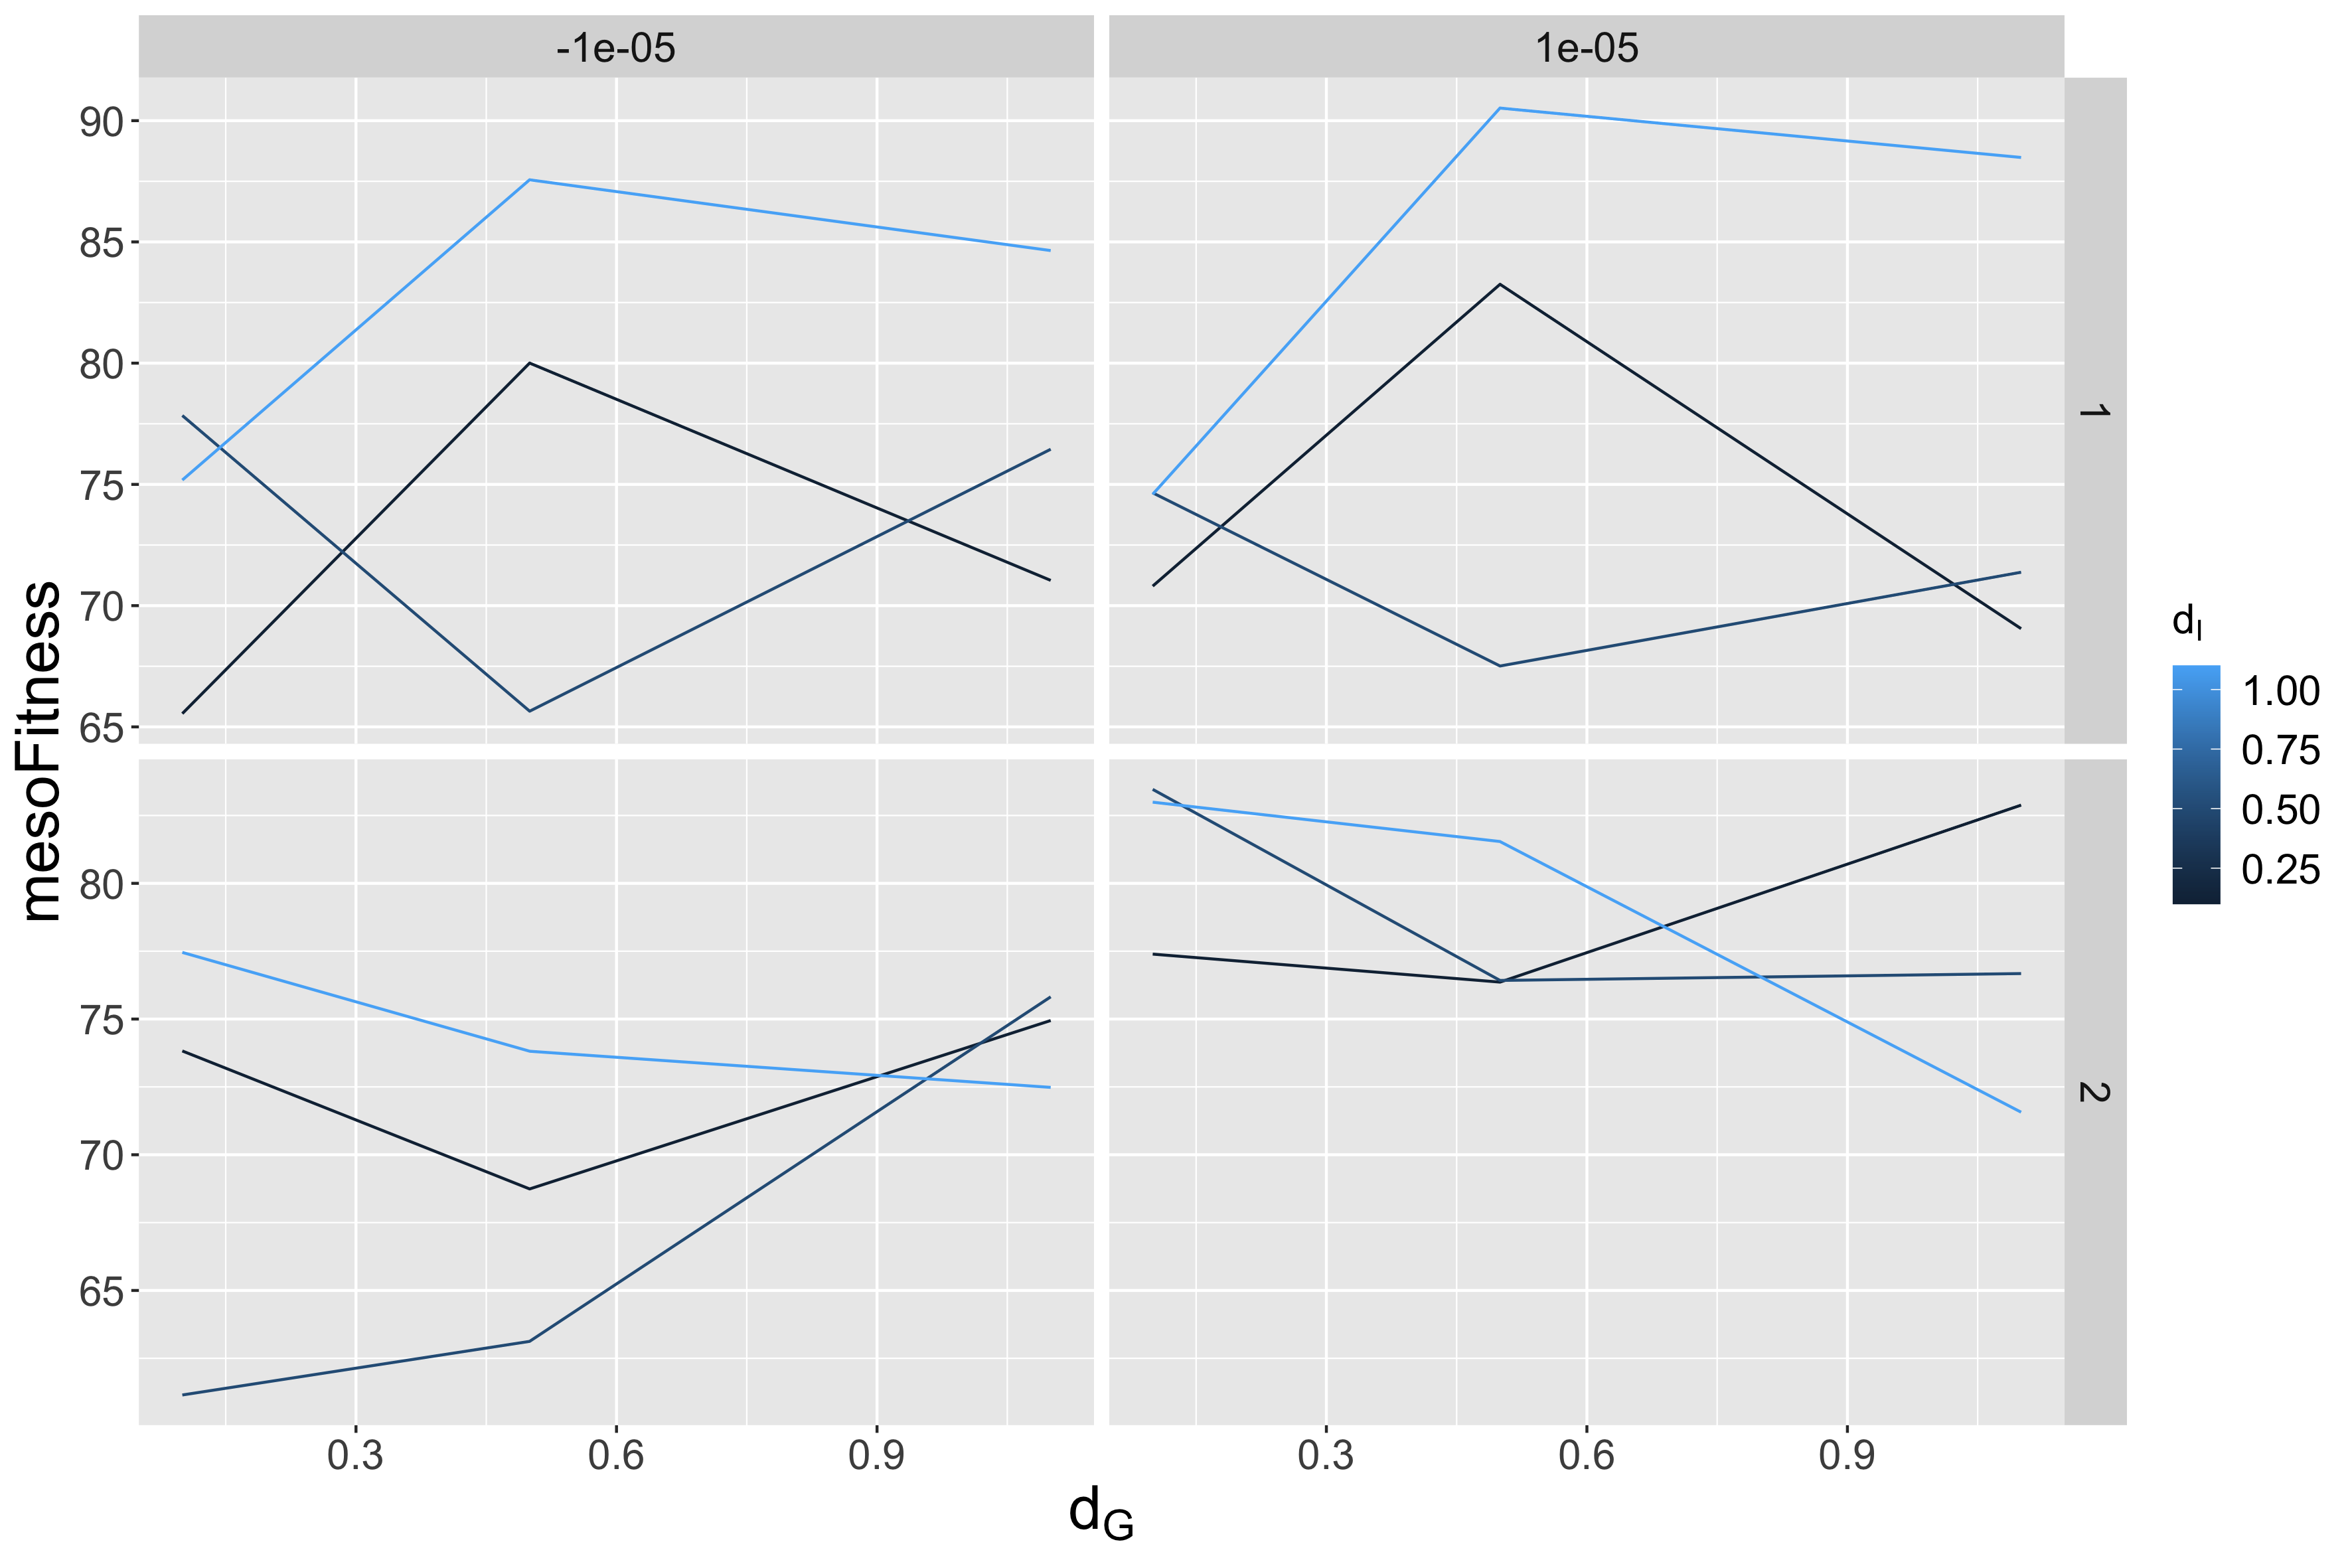
\includegraphics[width=\linewidth]{figures/mesoFitness-macroGravityDecay_color-macroInnovationDecay_facet-mesoToMacroInnovationThreshold-macroToMesoExchangeMaxUpdate_mesoCrossOverProba05.png}
    \caption{Behaviour of macro utility and meso fitness as a function of $d_G$, for varying $d_I$ (colour), $\beta_E$ (columns) and $\theta$ (rows).\label{fig:explo}}
\end{figure*}

\subsection{Statistical behavior}

% - statistical valid: LSH with many replications
% ! rerun simus on grid

We first test the statistical behavior of the model, in particular how much repetitions are needed to have a reasonable estimation of indicators. We explore a grid of 288 parameter points, and run 20 repetitions of the model on each. Estimating Sharpe ratios as the ratio between estimated mean and estimated standard deviation over the repetitions, we obtain across all macro and meso indicators all median ratios above or around 2, and a minimum across parameter points of 0.858 for the macro utility. Looking at all distance between couples of indicator averages, normalised by standard deviations (capturing the overlap between effect difference and standard errors), we find a minimal median of 0.19 for meso diversity, while other indicators have a median between 0.24 and 0.3. This means a rather good statistical separability of parameter points, and that 10 repetitions are enough for the stochastic variability to induce smaller noise than confidence intervals for averages.

\subsection{Grid exploration}

% - grid explo or one-factor ?

We then turn to a grid exploration of a portion of the parameter space, to understand some aspects of model behavior. We fix $p_M = 0.01$, $p_E=1e-4$, $\beta_C=0.0$, $\beta_M=0.0$ and take $(d_G,d_I)\in \{0.1,0.5,1.1\}$; $p_C \in \{0.2, 0.5\}$; $\theta \in \{1 , 2\}$; $\beta_E \in \{-1e-4 , 1e-4\}$.



We draw some plots of indicator behaviour in Fig.~\ref{fig:explo}. We find that the feedback parameter on the urban environment $\beta_E$ has a qualitative influence on the macro utility: while having comparatively small variations for negative values (left column), it becomes either strongly decreasing ($\theta=1$) or increasing ($\theta=2$) as a function of $d_G$. This implies that policies can in some cases reverse the effect of geography, what would correspond to voluntary development of stagnating regions. The role of $d_I$ also qualitatively changes, meaning that the distance of exchanges will affect differently interventions. A diversity of behaviours is also observed for the meso fitness. For both levels, $\theta$ also strongly changes qualitative behaviours - meaning that thresholds to access the market have in the end a long term impact on the overall system. Altogether, the influence of both feedback parameter can not be intuited from the beginning, and this first exploration allows diving in the complexity of model dynamics.

\subsection{Multi-objective optimisation}

% - multi-obj optimisation : global U vs companies? utility / diversity?

We then apply our model to a contradictory optimisation exercise. Often in such multi-scalar systems, actors and processes at different scales have different interests and can be in opposition. Solving such disputes is the objective of such integrative modeling approaches. We propose thus to simultaneously optimise the macroscopic utility, while still maximising the mesoscopic diversity. Previous exploration of the macro model showed that a compromise existed between macro utility and diversity; we try now to see if a similar one exist between scales. The diversity of ideas is an important aspect to be maintained for the resilience and innovativity of social systems, and can in some cases be hindered by global productivity objectives.

We run a NSGA2 bi-objective algorithm, for 10000 generations, with a population of 200 individuals, with as a genome the free parameter boundaries given above. We use the OpenMOLE implementation of NSGA2. The Pareto front obtained is shown in Fig.~\ref{fig:pareto}.

\begin{figure}[h!]
    \centering
    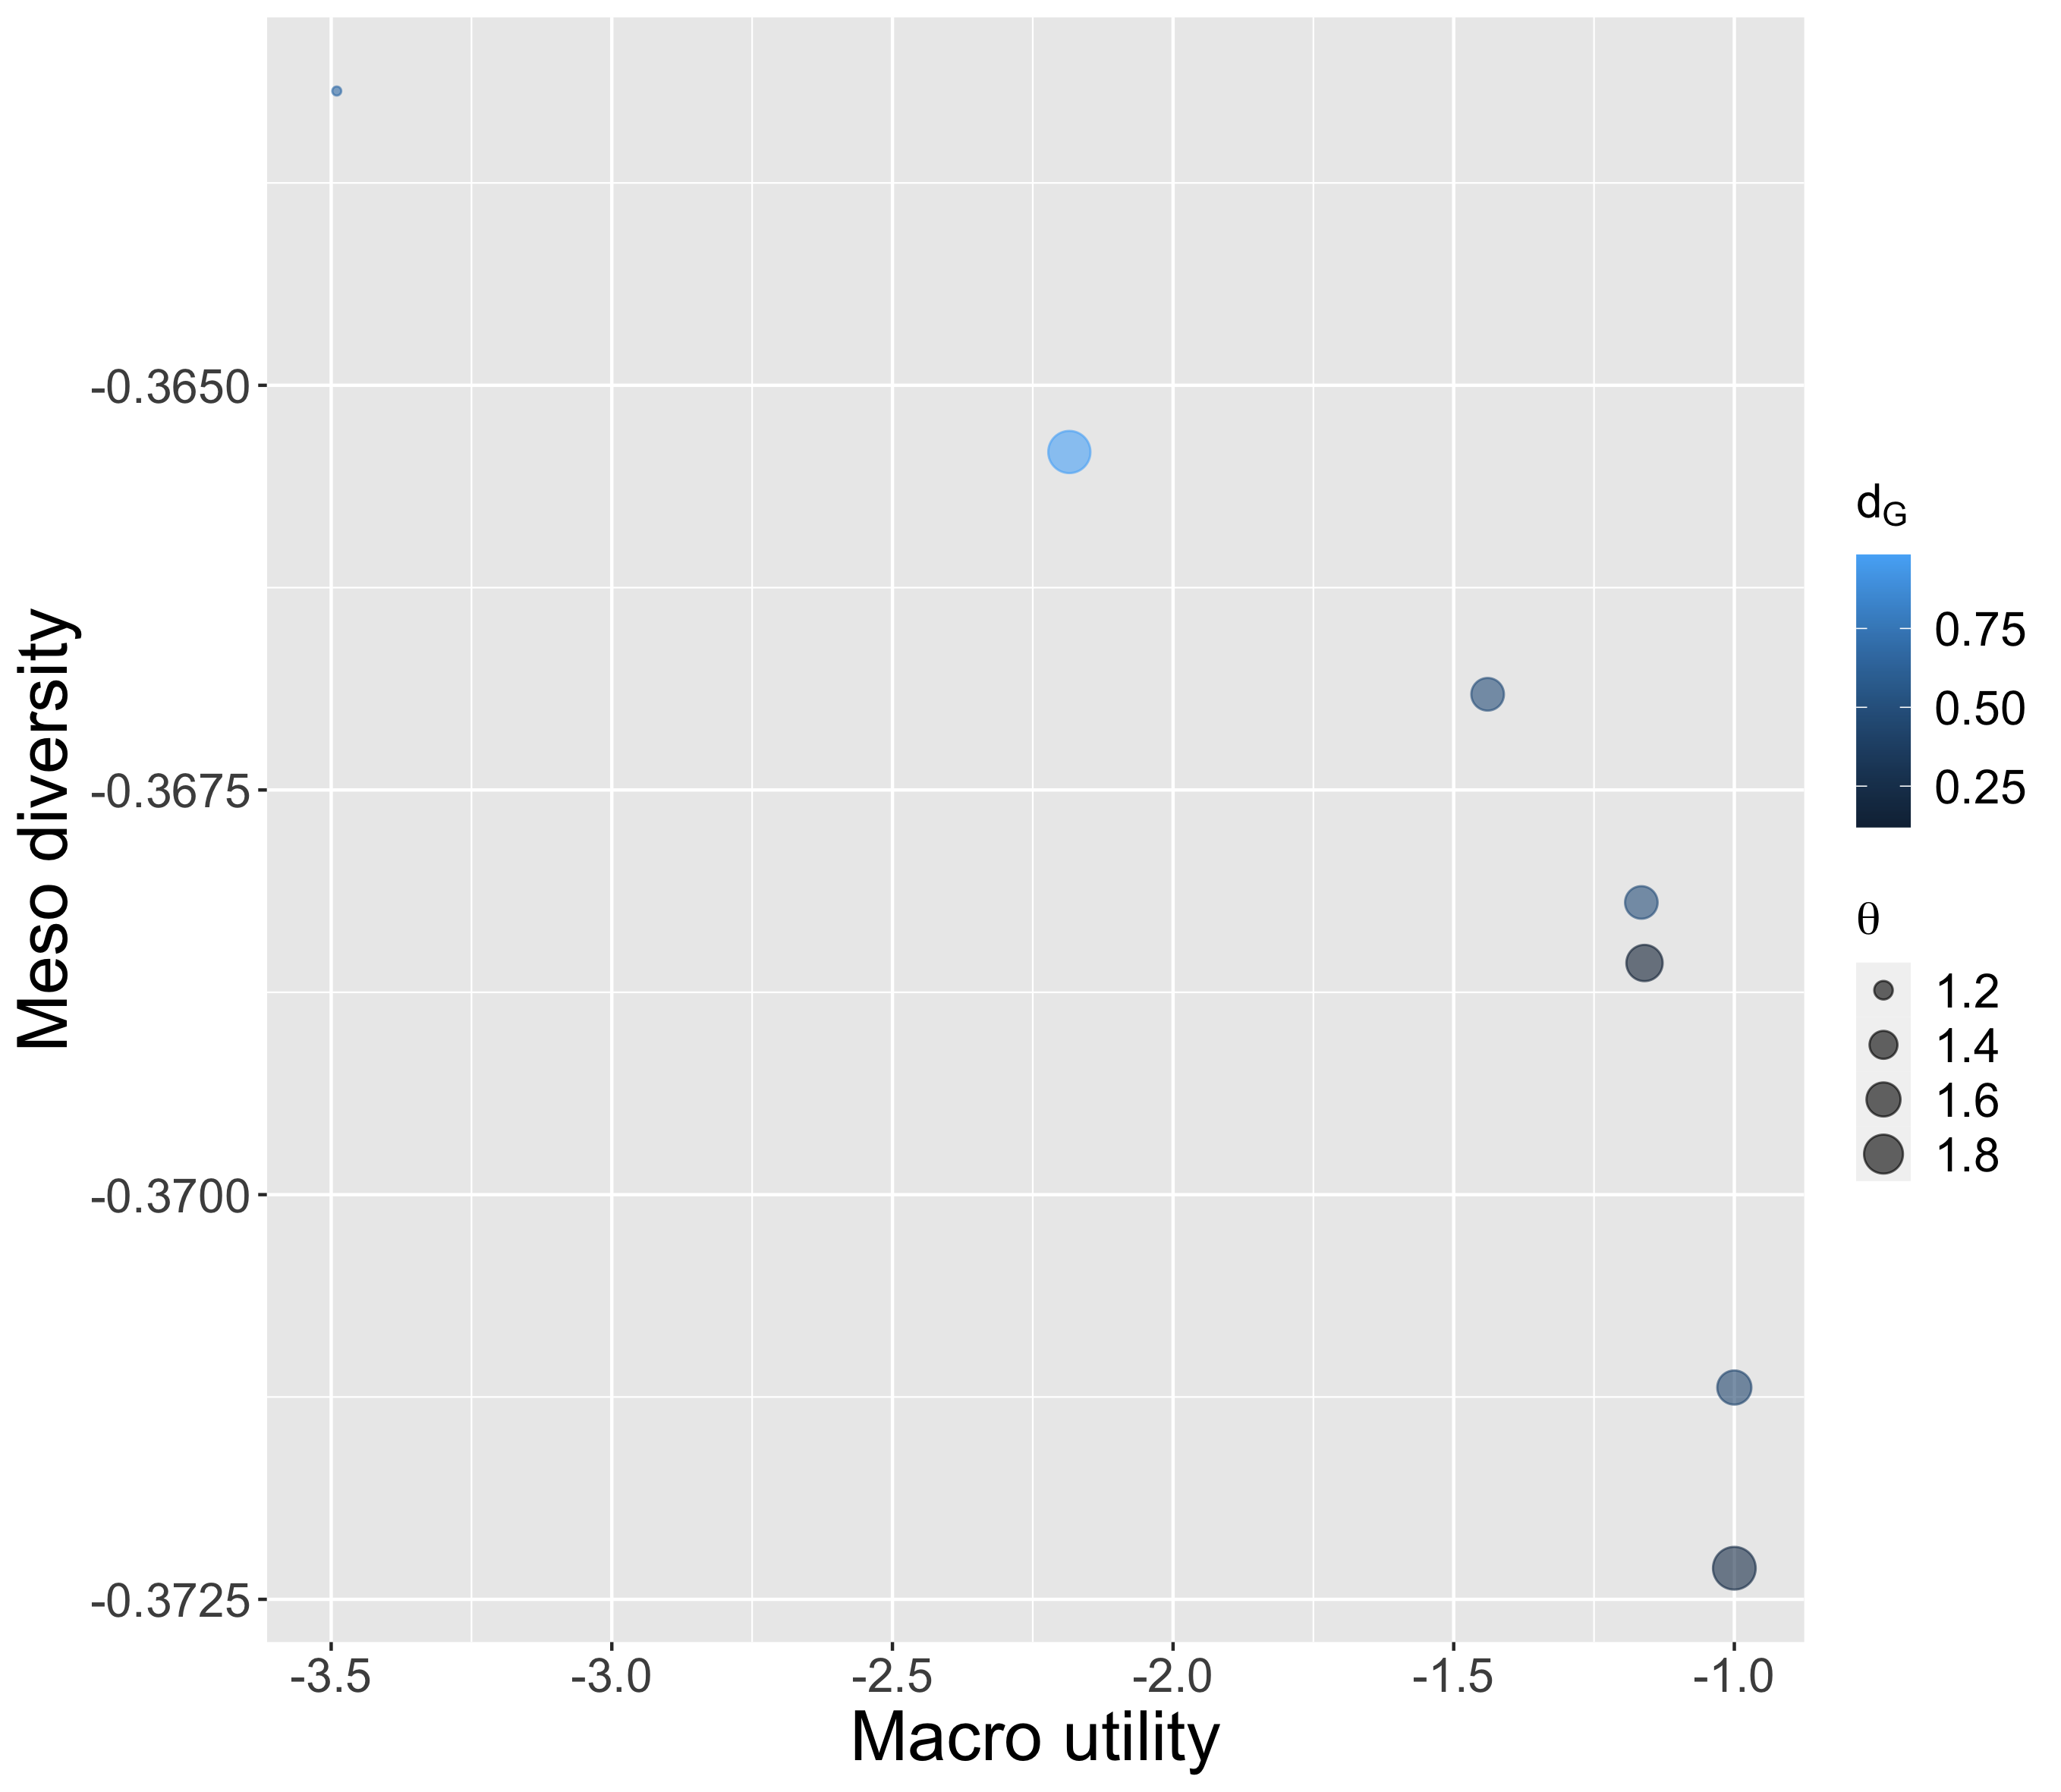
\includegraphics[width=\linewidth]{figures/paretoDiversity-Fitness_colordG_sizetheta}
    \caption{Pareto front between the opposite of macro utility and the opposite of meso diversity (both to be minimised to maximise the original objectives). Point color gives interaction distance $d_G$ and point size the innovation threshold $\theta$.\label{fig:pareto}}
\end{figure}

We find first of all a reduced number of points (10), suggesting that the optimisation is difficult. They however form a Pareto front, with a concave shape - on the contrary to convex fronts generally obtained. This means that extreme points are rather good compromises, witnessing very different regimes which can lead to optima. A middle point corresponds to long interaction distances (large $d_G$), while some points around and on the right extremity of the front are local regimes (small $d_G$), what could be evidence for a detrimental globalisation in that case. It is also a regime where innovation threshold is high, corresponding to a more competitive environment. This optimisation exercise confirms that both scales can be simultaneously taken into account and optimised in policy design.


\subsection{Searching for diversity in regimes of emergence}

% - specific experiment for downard causation : indicator? -> search with PSE?

We finally use the downward causation indicators to investigate which kind of emergence the model produces. We apply the PSE (Pattern Space Exploration) algorithm, implemented in OpenMOLE by \cite{cherel2015beyond}, and which is a hitmap-based diversity search algorithm, to explore the feasible space of these indicators. We run the algorithm for 10000 generations, with 3 objectives $\Psi (U)$, $\Delta (U)$, $\Gamma (U)$, the downward causation indicators on macro utility.


\begin{figure}[h!]
    \centering
    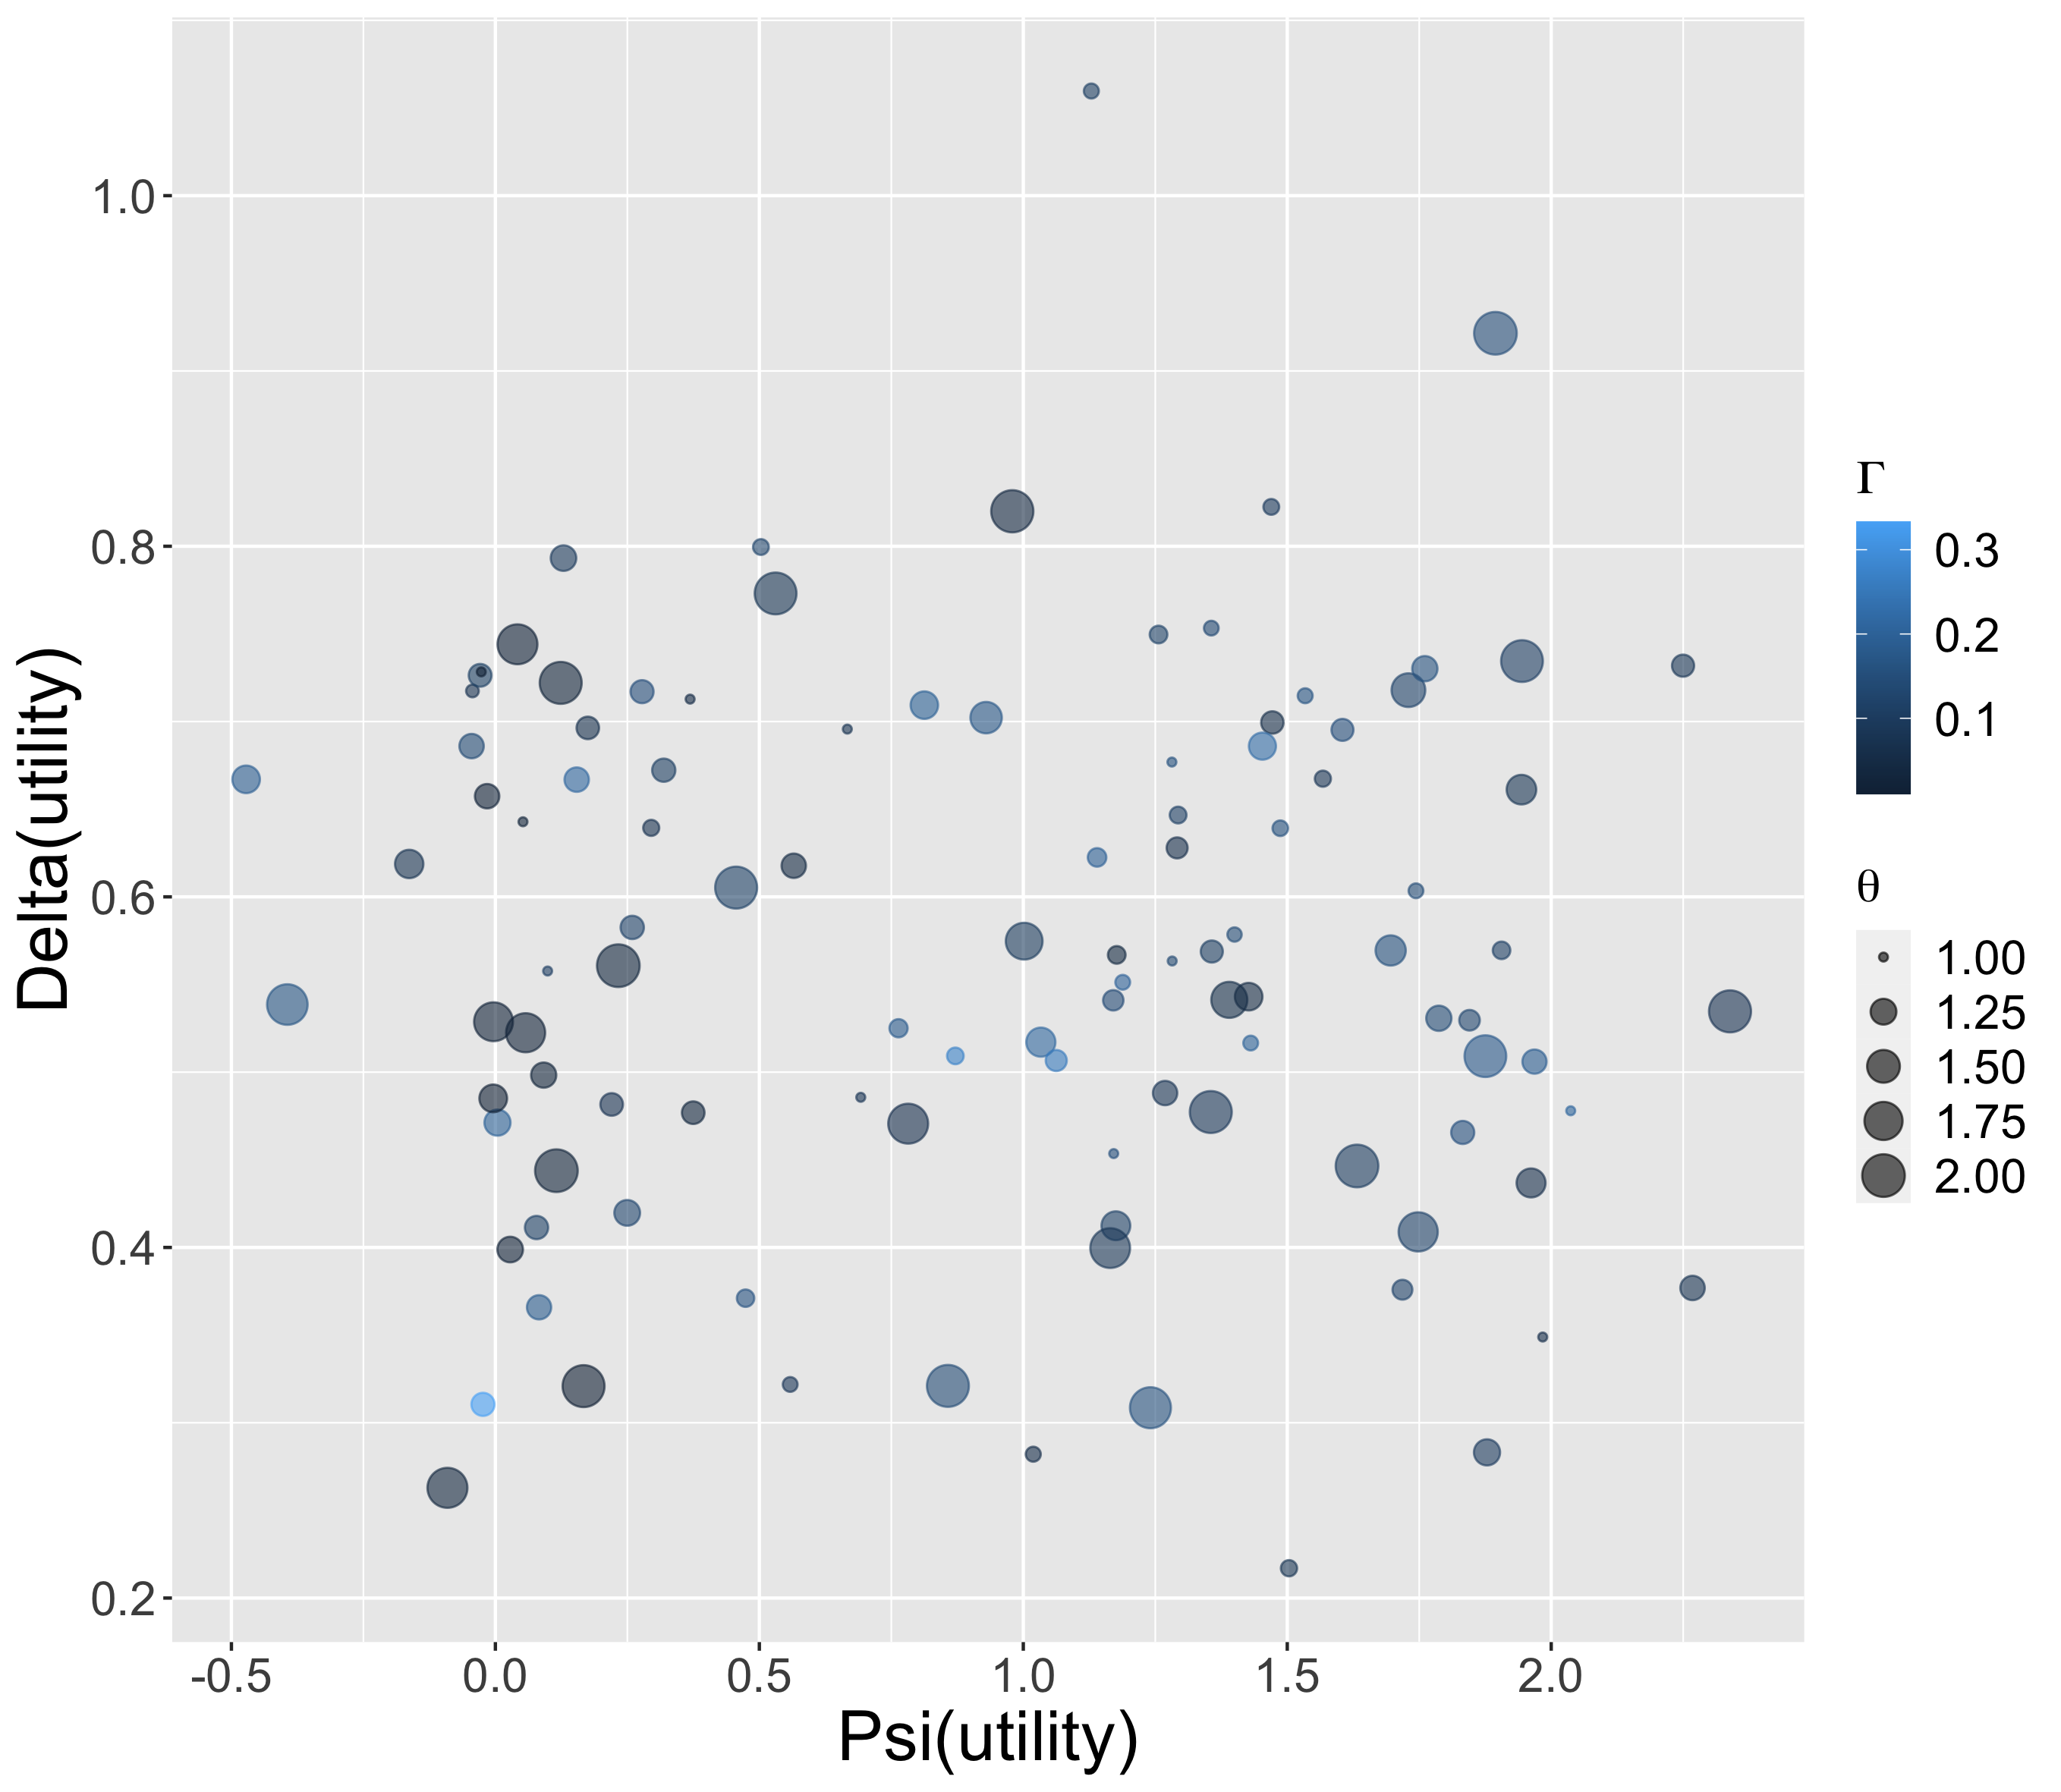
\includegraphics[width=\linewidth]{figures/pse-psi-delta-utility_colorGamma_sizetheta.png}
    \caption{Scatter plot between $\Psi (U)$ and $\Delta (U)$, obtained with the PSE diversity search algorithm. Point colour gives $\Gamma (U)$ and point size the innovation threshold $\theta$.\label{fig:pse}}
\end{figure}

The point cloud obtained is shown in Fig.~\ref{fig:pse}. We find a rather covering cloud, meaning that the model covers a great variety of regimes of emergence. A part of the points are gathered around $\Psi \sim 0$ for varying $\Delta$, corresponding to cases with no causal emergence but downward causation. Several points, disseminated across the cloud, have a value of $\Gamma$ close to 0, implying an autonomy between scale for the positive $\Psi$. $\Delta$ is never negative nor close to 0, meaning that downward causation always occurs, what could have been expected through the explicit top-down feedback process. Altogether, this last experiments confirms that the model captures strong emergence, but also a great variety of causal regimes between scales.


\section{Discussion}

% // empirical literature clusters

% link between scales done via policies!

% Limits
% - one dim product/utility space : // circeco
% - eco structure simple -> // abmfirms
% synthetic systems -> first level-specific data driven (not done yet) to be able to have multiscale data-driven? ~
% - migration between (and within) meso states : d_G? ; pop driven vs skill driven? - NOT IMPLEMENTED -> discuss why ok - reinit of optim at each cycle; sizes should evolve? ~ ->  \cite{hoisl2017r} role of diversity, many factors, larger size more complex projects, but in time: ?

% developments
%  - heterogeneity and dynamics of theta (meso -> macro)
%  - no change in macro params and uniform -> could fo as for multiscale urban form
% space matters

%- discuter cycle meso : reinit; nombre de firmes scale -> chance d'innover aussi? clarifier relations

% - more tests for downward causation - other delays

% possibilities top-down feedback
%    * H1 product adaptation: demand -> meso utility ; pb: how to compute utility - no economic model for demand
%    * H2 breakthrough innovation : firms explore far from mainstream? ~ -> include diversity in meso genetic algorithm
%    * H3 macro pop+innov influence (p_C,s_c) and (p_M, x_M) => firm strategy responding to urban dynamics: ex relocate certain activities, projects in dynamic areas - induce more chge
%    * H4 macro pop+innov influence (p_E, d_E): modification of the urban environment

We have introduced a multi-scalar model for innovation dynamics in systems of cities. Our numerical experiments show, beyond basic model validation and exploration, that (i) contradictory objectives can be optimised through policies across scales, suggesting that this type of approach could further be explored for territorial sustainability; (ii) strong emergence and a great diversity of emergence regimes are captured by the model - confirming the relevance of strongly coupling scale and building such a ``complicated'' model, beyond a single scale.

Several limits can at this stage be identified, and should be considered for future extensions. The unidimensional innovation space is a strong limitation, keeping the model abstract and difficult to link with data. The economic structure and processes is also very simplified, as we are closer to a phenomenological model. Coupling with economic agent-based models is a perspective for this issue. Regarding the time scales and evolution of urban areas, we also did not include migration of employees - assuming constant team sizes - what is fine with the idea of reinitialised settings at each macro time step, but what would cause more problems if we add memories to companies and employees. In that context, team diversity is crucial for innovation, but the role of sizes and their evolution in time is less clear \citep{hoisl2017r} - so translating population migration directly into firm sizes may not be the best solution. We did not include changes in macro parameters as \cite{raimbault2021strong} does, what could be a way to incorporate more bottom-up feedback in the model.

Finally, future developments on empirical data would need some model adaptation and complicated data collection and processing work. In particular, finding proxies for innovation, and also collecting firm data which is quite rare, are crucial issues. Such an empirical approach would however be necessary for real-world applications of the model beyond stylised policies.

\section{Conclusion}

This work introduced a first modelling and simulation step towards multi-scalar quantitative approaches to systems of cities, focused on innovation dynamics in this case. The numerical explorations, achieved with advanced model validation techniques with the OpenMOLE software, confirm the relevance of the model, in particular through its ability to capture a diversity of emergence regimes. This provides a first step towards more elaborated integrated urban models for sustainable policies.



\footnotesize
\bibliographystyle{apalike}
\bibliography{biblio}


\end{document}


% Template

\begin{figure}[t]
\begin{center}
\includegraphics[width=2.1in,angle=-90]{fig1.eps}
\caption{``Energies'' (inferiorities) of strings in a first-order
  phase transition with latent heat $\Delta\epsilon$.}
\label{fig1}
\end{center}
\end{figure}


\begin{table}[h]
\center{
\begin{tabular}{|c|c|c|c|}\hline
Name & Result & Bonus $b_i$ & Difficulty\\ \hline\hline
Echo & I/O   & 1 & --\\
Not  & $\neg A$ & 2 & 1 \\
Nand & $\neg(A\wedge B)$ & 2 & 1 \\
Not Or & $\neg A \vee B$ & 3 & 2 \\
And  &  $ A \wedge B $   & 3 & 2 \\
Or   &  $ A \vee B $     & 4 & 3 \\
And Not & $A\wedge\neg B$& 4 & 3 \\
Nor  & $\neg(A\vee B)$   & 5 & 4 \\
Xor  & $ A\ {\rm xor}\ B$ &   6 & 4 \\
Equals &$\neg(A\ {\rm xor}\ B)$&6& 4 \\ \hline
\end{tabular}
}
\vskip 0.25cm
\caption{Logical calculations on random inputs $A$ and $B$ rewarded,
bonuses, and difficulty (in minimum number of {\tt nand} instructions
required). Bonuses $b_i$ increase the speed of a CPU by a factor
$\nu_i=1+2^{b_i-3}$.}
\end{table}
